\documentclass[ex,minted]{exercise}

\deadline{12.12.2023}

\begin{document}

\section{Kerr-Effekt Messung}
Der Geschwindigkeitsunterschied zwischen dem ordentlichen und außerordentlichen 
Strahlen eines Laser mit einer Wellenl¨ange von $\lambda = 550 \u{nm}$ in einer 
Kerr-Zell betr¨agt 2\textperthousand{} der Lichtgeschwindigkeit im Vakuum. Dabei wurde ein
homogenes E-Feld mit einer St¨arke von $\abs E = 5 \cdot 10^5 \ufrac Vm$
angelegt. Der mittlere Brechungsindex der Zelle betr¨agt
$n = 1.553$. Bestimmen Sie die Kerr-Konstante $K$.

\dottedlinete

\begin{align*}
    \Delta n &= K \lambda E^2
\end{align*}\tight
\begin{align*}
    K &= \frac{\Delta n}{\lambda E^2}
    = \frac{1.553\cdot(1.002 - 1)}{550\u{nm} \cdot \hug{5\E5\ufrac Vm}^2}
    \approx 22.6\E{-9}\ufrac{m}{V}
\end{align*}

\section{Stehende Elektronenwelle}
Stellen Sie sich vor Sie halten ein Elektron in einem 1-dimensionalen "Kasten" mit einer 
Kantenlänge \(L=1\u{cm}\). Welchen Impulsen entsprechen stehende De-Broglie-Wellen?

\dottedlinett

Nur die folgenden Wellenlängen erfüllen die durch den Kasten 
vorgegebenen Randbedingungen:
\begin{align*}
    \lambda_n &=  \frac{2L}{n} \note n\in\N_0
\end{align*}
Die dazugehörigen Impulse sind:
\begin{align*}
    p_n &= \frac{h}{\lambda_n} = \frac{n \,h}{2L}
\end{align*}

\section{Photoeffekt}
In der Vorlesung wurde der Photoeffekt an einer Photoröhre beobachtet, deren Kathode
mit dem Licht von fünf verschiedenen Wellenlängen bestrahlt wurde. Es wurde jeweils die 
Gegenspannung \(U_g\) gemessen, die den Photostrom zum Verschwinden brachte. In einer 
anderen Messreihe mit dem gleichen Aufbau erhielten wir folgende Werte: 
\begin{center}
    \begin{tabular}{c|ccccc}
        $\lambda[\u{nm}]$ & 405 & 465&505&590&625\\\hline
        $U_g[\mathrm V]$ &1.4&1.25&0.85&0.2&0.15
    \end{tabular}
\end{center}
Tragen Sie die Messung geeignet auf und ermitteln Sie die Austrittsarbeit \(A\), das 
Verhältnis \(h/e\) und die Grenzfrequenz \(\nu_g\). Schätzen Sie auch jeweils 
deren Fehler ab. Nehmen Sie dabei für die Spannungsmessung einen Fehler 
von \(0.1\u V\) an. Den Fehler auf die Wellenlänge können Sie vernachlässigen.

\dottedlinett

Aus der Energiebilanz geht hervor, dass:
\begin{align*}
    A &= E_{\te{ph}} - E_{\te{el}} 
    = \frac{h}{\lambda}- e U_g = 
    h\,f - e U_g \\
    e U_g &= h\,f-A
\end{align*}


\inputpy{Python-Code}{9.py}

\begin{figure}[H]
    \centering
    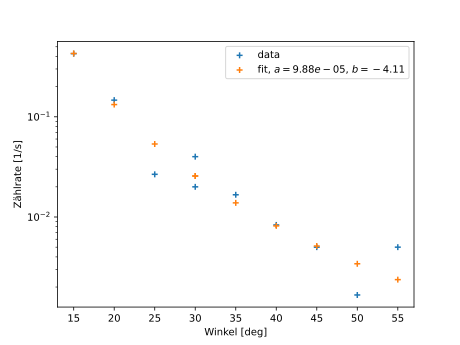
\includegraphics[width=0.7\textwidth]{2.png}
    \caption{Resultierender Plot}
\end{figure}

Die durch den Fit ermittelten Werte sind
\begin{align*}
    h &= (8.526\pm1.285)\E{-34} \u{Js}\\
    A &= (2.387\pm0.482) \u{eV}\\
    h/e &= (5.322\pm0.802)\E{-15} \ufrac{Js}{C}\\
    \nu_g &= (4.486\pm1.130)\E{14} \ufrac1s 
\end{align*}


\section{Das Experiment von Davisson und Germer}
\subsection{Erklären Sie die auf S.723 des obigen Artikels genannte "grating formula": 
\(n\lambda = d\sin\theta\)}

\dottedlinett

Das "grating formula"{} lässt sich herleiten, indem man annimmt, dass das
Licht nur an den annäherungsweise punktförmigen Atomen refektiert wird. 
Das Licht zwischen zwei benachbarten Atomen hat unter dem Winkel 
\(\theta\) einen konstanten Wegunterschied \(\Delta s\),
den man durch Betrachtung der Geometrie als \(\Delta s = d\sin\theta\)
bestimmen kann. 

\begin{figure}[H]
    \centering
    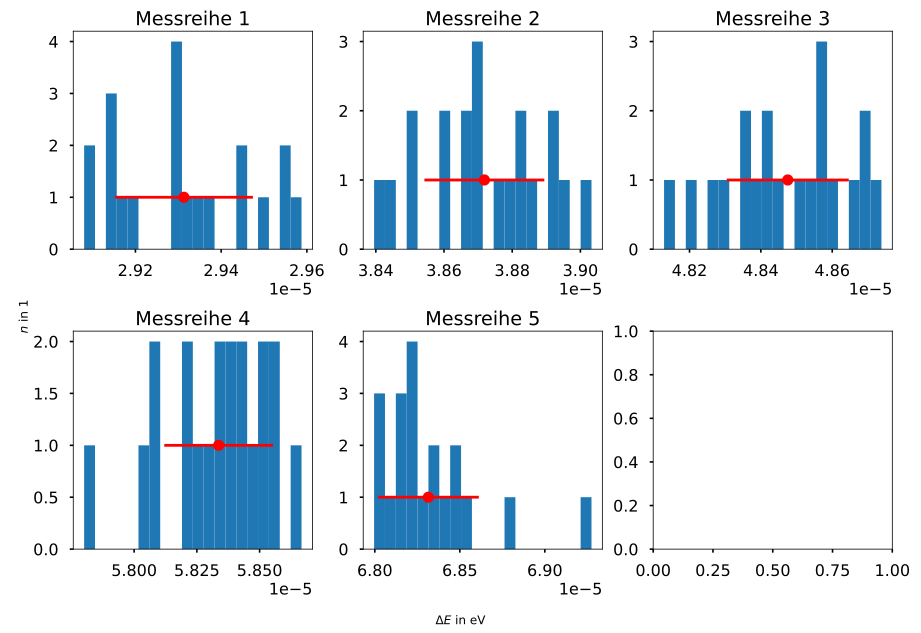
\includegraphics[width=0.7\textwidth]{1.png}
    \caption{Skizze des Kristalls und der Reflexion.}
\end{figure}

Die Skizze zeigt den Aufbau, der Wegunterschied ist eingezeichnet.
An einem Beugungsmaximum muss der Wegunterschied \(\Delta s = n\lambda\) sein,
damit konstruktive Interferenz auftritt. Insgesamt ergibt sich also für die 
Winkel der Maxima \(n\lambda = d\sin\theta\).

\subsection{Erklären Sie die Formel auf S.722 in Table 1 für die 'equivalent wavelength':
\(\lambda=\sqrt{150/V}\)}

\dottedlinett

Aus der Energiebilanz der Elektronen nach durchlaufen der Beschleunignungsspannung
lässt sich die Geschwindigkeit und damit der Impuls herleiten:
\begin{align*}
    E_{\te{kin}} &= E_{\te{el}}\\
    \frac 12 mv^2 &= e U \\
    v &= \sqrt{\frac{2 e U}{m}} \\
    p &= \sqrt{2 m e U}
\end{align*}

Die zugehörige De-Broglie-Wellenlänge ist:
\begin{align*}
    \lambda &= \frac{h}{p} \\
    &= \frac{h}{\sqrt{2 m e U}}\\
    &= \frac{\ch}{\sqrt{2 \cdot \cme \cdot\ce \cdot U}} \\
    & \approx \sqrt{1.51\E{-18} /U}\\
    &= 10^{-10}\sqrt{151/U}\\
    &= \sqrt{151/U} \for \lambda \te{ gemessen in \r A}
\end{align*}

Die Formel beschreibt also die De-Broglie-Wellenlänge (\r A) der Materiewelle 
in Abhängigkeit zu der Beschleunignungsspannung (V).

\subsection{Berechnen Sie nun den Gitterabstand des Nickel-Atomgitters, an dem
die Beugung erfolgte.}

\dottedlinete

\begin{align*}
    n\lambda &= d\sin\theta\\
    n \sqrt{151/U} &= d\sin\theta\\
    d &= \frac{n \sqrt{151/U}}{\sin\theta}\\
    &= \frac{1\cdot \sqrt{151/54\u V}}{\sin 50^\circ}\\
    &= 2.18 \te{\r A}
\end{align*}
\end{document}